\section{Task 2}

\subsection{1}
Vi bliver bedt om at løse nedenstående rekursion ved substitution.
\begin{equation*}
	p(n) = p(\frac{n}{2}) + p(\frac{n}{3}) + n
\end{equation*}
For at komme frem til et gæt på en løsning vil vi tegne rekursionstræet:
\begin{figure}[h]
	\centering
	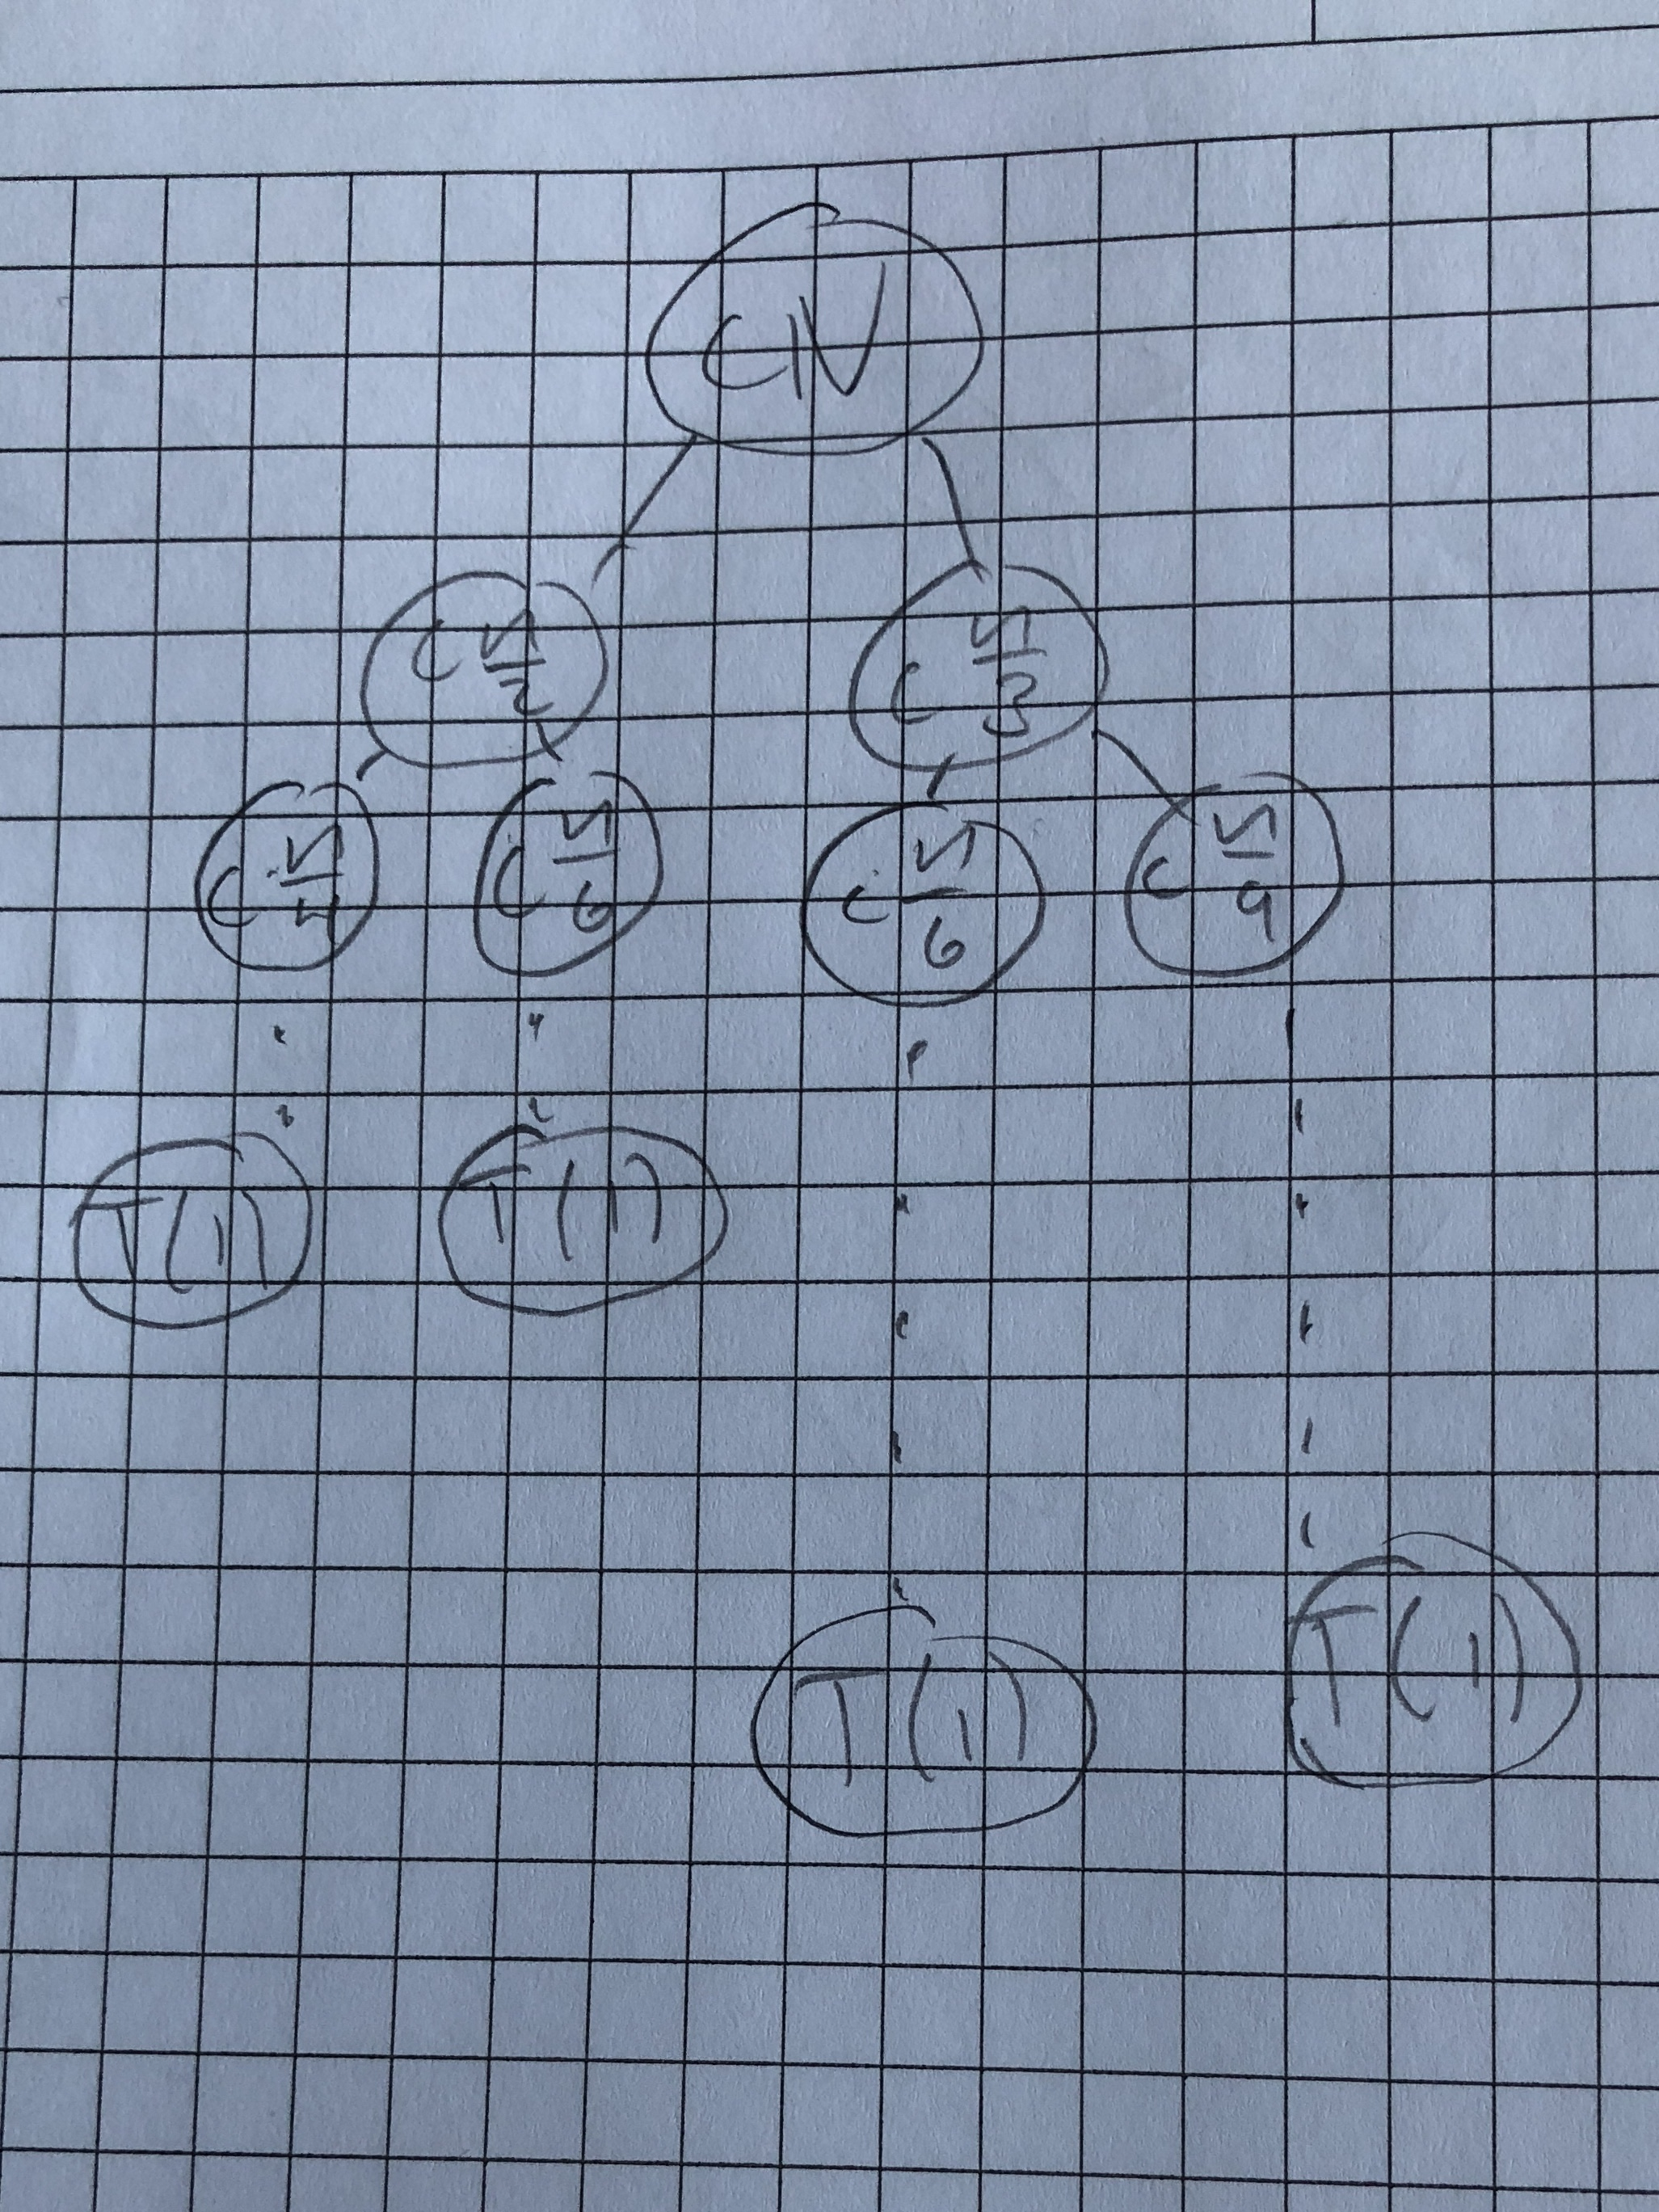
\includegraphics[height=15cm]{Materials/RecTree}
\end{figure}

Som det ses på træet, så har vi en geometrisk serie. Denne kan omskrives til en sum som følger\footnote{Introduction to algorithms - s. 90}:
\begin{align*}
	T(n) &= \left(cn\left(\frac{5}{6}\right)^0 + cn\left(\frac{5}{6}\right)^1 + \cdots + cn\left(\frac{5}{6}\right)^{log_2(n)} + cn\left(\frac{2}{6}\right)^{log_2(n)+1} + \cdots + cn\left(\frac{2}{6}\right)^{log_3(n)}\right)  \cdot log(n)\\
	&\leq \left(cn\left(\frac{5}{6}\right)^0 + cn\left(\frac{5}{6}\right)^1 + \cdots + cn\left(\frac{5}{6}\right)^{log_3(n)}\right) \cdot log(n)\\
	&= \sum_{i = 0}^{log_{3}(n-1)}\left(\frac{5}{6}\right)^icn \cdot log(n)\\
	&\leq \sum_{i = 0}^{\infty}\left(\frac{5}{6}\right)^icn \cdot log(n)\\
	&= \frac{1}{1-\frac{5}{6}}cn \cdot log(n)\\
	&= 6n\cdot log(n)\\
	&= O(nlog(n))
\end{align*}

Vi har nu et gæt og kan gå i gang med vores bevis.\\
Vi vil nu gerne vise at for $P(n) = P(n/2) + P(n/3) + n$:
\begin{equation*}
	P(n) \leq cnlog(n)
\end{equation*}
Vi kan nu begynde beviset ved at substituere ind:
\begin{align*}
	P(n) &\leq c(n/2)log(n/2) + c(n/3)log(n/3) + n\\
	&\leq c(n/2)log(n/2) + c(n/3)log(n/2) + n\\
	&\leq cnlog(n/2) + n\\
	&= cnlog(n) + cnlog(2) + n\\
\end{align*}

Vi kan nu se at hvis $cnlog(2) + n \geq 0$, så holder vores ulighed. Ved at løse for c finder vi:
\begin{align*}
	cnlog(2) + n &\geq 0\\
	cnlog(2) &\geq -n\\
	c &\geq \frac{-1}{log(2)}
\end{align*}

Vi har dermed bevist at for $c \geq \frac{-1}{log(2)}$ holder vores ulighed for alle $n \geq n_0$ (Dog bemærkes det, at $\frac{-1}{log(2)} < 0$ og $c$ pr. definition skal være skaprt større end nul, således at uligheden i realiteten kun gælder for alle $c > 0$), og er derfor $P(n) = O(nlog(n))$.

\subsection{2}

$p(n) = \sqrt(n)p(\sqrt(n)) + \sqrt(n)$\\
Vi omskriver $p(n)$ til noget simplere ved at lade $m = lg(n)$:
$$p(2^m) = 2^{\frac{m}{2}}p(2^{\frac{m}{2}}) + 2^{\frac{m}{2}}$$
Dernæst definerer vi en ny reccurence givet ved $s(m) = p(2^m)$:
$$s(m) = 2^{\frac{m}{2}}p(\frac{m}{2}) + 2^{\frac{m}{2}}$$
Vi genkender, at $s(m)$ har løsningen $s(m) = O(2^mlg(m))$ (som det fremgår i CLRS side 87).
Dvs:
$$p(n) = p(2^m) = s(m) = O(2^mlg(m)) = O(nlg(lg(n)))$$
